\subsection{Architecture}
ECDAR consists of five major components seen in \autoref{fig:ECDAR-architecture}.
These componenets are the two engines: Reveaal and j-Ecdar, ECDAR GUI, its test framework, and its communication between the engines and GUI: Protocall buffer.
\begin{figure}[H]
    \centering
    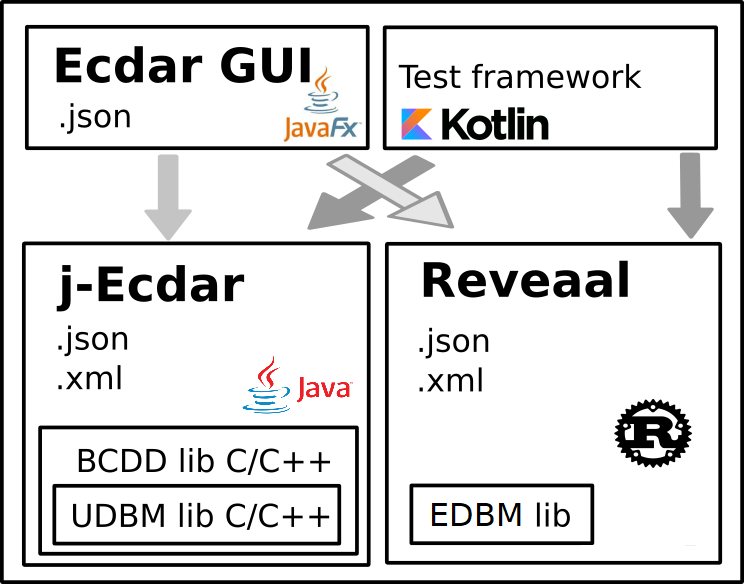
\includegraphics[width=0.75\textwidth]{common/figures/ArchOverview.png}
    \caption{The architecture of ECDAR visualized \cite{ECDARNET}.}
    \label{fig:ECDAR-architecture}
\end{figure}
%Figure old, get new
The graphical user interface (\textbf{GUI}) is written in JavaFX which is a set graphics and media library for Java. The interface provides the tools which enables the user to model their real time systems. The interface sends queries to the engines through gRPC (\textbf{G}oogle \textbf{R}emote \textbf{P}rocedure \textbf{C}all) using protocall buffers. This is illustrated by the arrows going from the Ecdar GUI component to the j-Ecdar and Reveaal components as seen in \autoref{fig:ECDAR-architecture}. The gRPC framework has the advantage of being cross platform and works across languages \cite{gRPC}, simplifying the integration process and making it easy to use.

ECDAR runs on two verification engines, j-Ecdar and Reveaal. The purpose of having two different engines is to make the whole platform more reliable.

The j-Ecdar component is an engine written in the java programming language, and its focus is readability and correctness, and ``where no effort is put into optimizing the code for speed''.\cite{ECDARNET}

The Reveaal engine is written in the Rust programming language and is intended to be fast and parallelizable. A goal for the Reveaal engine is to be able to run on multiple cores on multiple machines. 

ECDAR makes use of a testing framework written in Kotlin. 
The testing framework uses a collection of test cases to test both of the engines. 
The testing framework is vital to ensure conformance testing between j-Ecdar and Reveaal as well as automated performance testing and hand-designed test cases. 